%%%%%%%%%%%%%%%%%%%%%%%%%%%%%%%%%%%%%%%%%
% Simple Sectioned Essay Template
% LaTeX Template
%
% This template has been downloaded from:
% http://www.latextemplates.com
%
% Note:
% The %\lipsum[#] commands throughout this template generate dummy text
% to fill the template out. These commands should all be removed when 
% writing essay content.
%
%%%%%%%%%%%%%%%%%%%%%%%%%%%%%%%%%%%%%%%%%

%----------------------------------------------------------------------------------------
%	PACKAGES AND OTHER DOCUMENT CONFIGURATIONS
%----------------------------------------------------------------------------------------

\documentclass[12pt]{article} % Default font size is 12pt, it can be changed here

\usepackage[spanish]{babel}%Para el español
\usepackage[utf8]{inputenc}%para los acentos
\usepackage{amsmath,amssymb,amsfonts,amsthm}
\usepackage{graphicx}
\usepackage{bbm}
\usepackage{textcomp}
\usepackage{amstext}

\usepackage{geometry} % Required to change the page size to A4
\geometry{a4paper} % Set the page size to be A4 as opposed to the default US Letter

\usepackage{graphicx} % Required for including pictures

\usepackage{float} % Allows putting an [H] in \begin{figure} to specify the exact location of the figure
\usepackage{wrapfig} % Allows in-line images such as the example fish picture

\linespread{1.2} % Line spacing

%\setlength\parindent{0pt} % Uncomment to remove all indentation from paragraphs

\graphicspath{{Imagenes/}} % Specifies the directory where pictures are stored

%\usepackage{tikz}
%%%<
%\usepackage[spanish]{babel}%Para el español
%\usepackage[utf8]{inputenc}
%\usepackage{verbatim}
\usepackage{listings}
%\usepackage{xcolor}


%\usepackage{times}
 
%\definecolor{dkgreen}{rgb}{0,0.6,0}

\lstset{
	language=C,
	literate=%
	{á}{{\'{a}}}1
	{é}{{\'{e}}}1
	{í}{{\'{i}}}1
	{ó}{{\'{o}}}1
	{ú}{{\'{u}}}1
	{ñ}{{\~{n}}}1
	{<}{{$<$}}1
	{>}{{$>$}}1,
	basicstyle=\footnotesize\ttfamily,
	keywordstyle=\bfseries, 
	comment=[l]{\;},%
	breaklines=true,
	prebreak = \raisebox{0ex}[0ex][0ex]{\ensuremath{\hookleftarrow}},
    }

\usepackage{framed}
\usepackage{tabularx,colortbl}
\usepackage{adjustbox}
\usepackage{pdflscape}

\begin{document}


%----------------------------------------------------------------------------------------
%	TITLE PAGE
%----------------------------------------------------------------------------------------

\begin{titlepage}
\newgeometry{left=1.5cm,right=1.5cm}

\newcommand{\HRule}{\rule{\linewidth}{0.5mm}} % Defines a new command for the horizontal lines, change thickness here

\center % Center everything on the page

\textsc{\LARGE Universidad Nacional de Córdoba}\\[1.5cm] % Name of your university/college
\textsc{\Large Informe Trabajo Final}\\[0.5cm] % Major heading such as course name
\textsc{\large Programación Concurrente}\\[0.5cm] % Minor heading such as course title

\HRule \\[0.4cm]
\Large{ \huge \bfseries Simulación de una red flexible de producción mediante Redes de Petri.}\par % Title of your document
\HRule \\[1.5cm]

\begin{minipage}{0.5\textwidth}
\begin{flushleft} \large
\emph{Autores:}\\
Esteban \textsc{Morales} (35.104.714)\\
Marino \textsc{Uboldi} (34.140.737)\\
Santiago \textsc{Salamandri} (35.177.596)\\
\end{flushleft}
\end{minipage}
~
\begin{minipage}{0.4\textwidth}
\begin{flushright} \large
\emph{Supervisor:} \\
Mgs. Orlando \textsc{Micolini}
\end{flushright}
\end{minipage}\\[4cm]

{\large \today}\\[3cm] % Date, change the \today to a set date if you want to be precise

%\includegraphics{Logo}\\[1cm] % Include a department/university logo - this will require the graphicx package

\vfill % Fill the rest of the page with whitespace
\restoregeometry
\end{titlepage}

%----------------------------------------------------------------------------------------
%	TABLE OF CONTENTS
%----------------------------------------------------------------------------------------

\tableofcontents % Include a table of contents

\newpage % Begins the essay on a new page instead of on the same page as the table of contents 

%----------------------------------------------------------------------------------------
%	INTRODUCTION
%----------------------------------------------------------------------------------------

\section{Introducción} % Major section

En el presente informe se expone el desarrollo del trabajo final para la cátedra Programación Concurrente que se cursa en el primer cuatrimestre del cuarto año de la carrera Ingeniería en Computación en la Facultad de Ciencias Exáctas Físicas y Naturales de la Universidad Nacional de Córdoba, Argentina. 
Este trabajo tiene por consigna la simulación de una celda flexible de producción mediante el modelado por redes de petri y la implementación concurrente programada en Java. Tal implementación incluye la programación de los procesos productivos que ejecutan sus tareas de forma paralela y el diseño de un monitor para garantizar la sincronización de la adquisición y devolución de los recursos compartidos.  

%------------------------------------------------
\section{Consigna}
Sea una planta industrial donde se intenta producir tres tipos de piezas distintas mediante el uso de una celda de producción flexible que incluye tres robots, cuatro máquinas, tres almacenes de materiales y tres almacenes de piezas producidas.
Debe tener en cuenta las siguientes reglas de producción para cada pieza:
\begin{itemize}
\item \textsc{Pieza 1}: Para producir una unidad de pieza (1), una unidad de material del almacen $I_1$ debe someterse a los porcesos de la máquina $M_1$ y la máquina $M_2$. Finalmente se colocan las piezas producidas en el almacen $=O_1$.
$$I_1 \rightarrow M_1 \rightarrow M_2 \rightarrow O_1$$ 
\item \textsc{Pieza 2}: Existen dos reglas para producir una unidad de pieza (2), una unidad de material del almacen $I_2$ debe someterse a los porcesos de la máquina $M_4$ ,la máquina $M_3$ y la máquina $M_1$ ó bien pasar por las máquinas $M_2$, $M_3$ y $M_1$. Finalmente se colocan las piezas producidas en el almacen $=O_2$.
$$I_2 \rightarrow M_4 \rightarrow M_3 \rightarrow M_1 \rightarrow O_2$$
$$I_2 \rightarrow M_2 \rightarrow M_3 \rightarrow M_1 \rightarrow O_2$$
\item \textsc{Pieza 3}:Para producir una unidad de pieza (1), una unidad de material del almacen $I_3$ debe someterse a los porcesos de la máquina $M_3$ y la máquina $M_4$. Finalmente se colocan las piezas producidas en el almacen $=O_3$.
$$I_3 \rightarrow M_3 \rightarrow M_4 \rightarrow O_3$$ 
\end{itemize}
Los encargados de transportar los materiales, productos intermedios y finales son los robots, en este caso se cuenta con tres y cuyas responsabilidades se detallan a continuación:
\begin{itemize}
\item Robot 1 (R1):$[I_1,M_1,M_3,O_2]$
	\begin{itemize}
	\item Carga la máquina $M_1$.
	\item Libera la máquina $M_3$.
	\item Quita materiales del almacen $I_1$.
	\item Deposita las piezas (2) en el almacen $O_2$.
	\end{itemize}
\item Robot 2 (R2):$[I_3,M_1,M_2,M_3,M_4]$
	\begin{itemize}
	\item Libera la máquina $M_1$.
	\item Libera la máquina $M_2$.
	\item Libera la máquina $M_4$.
	\item Carga la máquina $M_3$.
	\item Carga la máquina $M_4$.
	\item Quita materiales del almacen $I_3$.
	\end{itemize}
\item Robot 3 (R3):$[M_2,M_4,0_1,0_3]$
	\begin{itemize}
	\item Carga la máquina $M_2$.
	\item Carga la máquina $M_4$.
	\item Libera la máquina $M_2$.
	\item Libera la máquina $M_4$.
	\item Deposita las piezas (1) en el almacen $O_1$.
	\item Deposita las piezas (3) en el almacen $O_3$.
	\end{itemize}
\end{itemize}
Se pide como consigna modelar el sistema con una red de petri, luego debe programarse la solución y emplearse un monitor para la sincronización de los procesos concurrentes.


%------------------------------------------------
\section{Red de Petri}
Una Red de Petri es uno de varios lenguages de modelado matemático para la descripción de sistemas distribuidos, paralelos y concurrentes. Una Red de Petri es un grafo bipartito, en el cual los nodos representan transiciones(eventos) y plazas(condiciones o estados), los arcos dirigidos indican cuales plazas son precondiciones y/o poscondiciones para la ejecución de una transición. 
Mediante la interpretación semántica de la consigna se produjo 3 redes de petri que describen los procesos productivos del sistema propuesto en la consigna.
3 IMAGENES
La ejecución de estas redes no presenta complicación alguna. Sin embargo al unirlas para construir la red completa del sistema aparecen deadlocks en la ejecución, interbloqueos producidos por el uso compartido de los recursos productivos.
1 IMAGEN
Seguidamente se analiza la circunstancia de interbloqueo de la red y es posible observar, con cierta facilidad, que el deadlock se produce cuando el segundo y el tercer proceso intentan producir cuatro piezas en simultáneo.
Naturalmente surge la idea de incorporar una restricción, la más obvia, limitar la producción simultanea de ambos procesos a sólo tres piezas.
Esta solución acaba con los interbloqueos y en ejecuciones posteriores no se observan deadlocks independientemente de la cantidad de pasos simulados.
Se muestra el modelo final de la red completa del sistema:
1 IMAGEN
\newpage
%\begin{landscape}
\begin{figure}[H] % Example image
\center{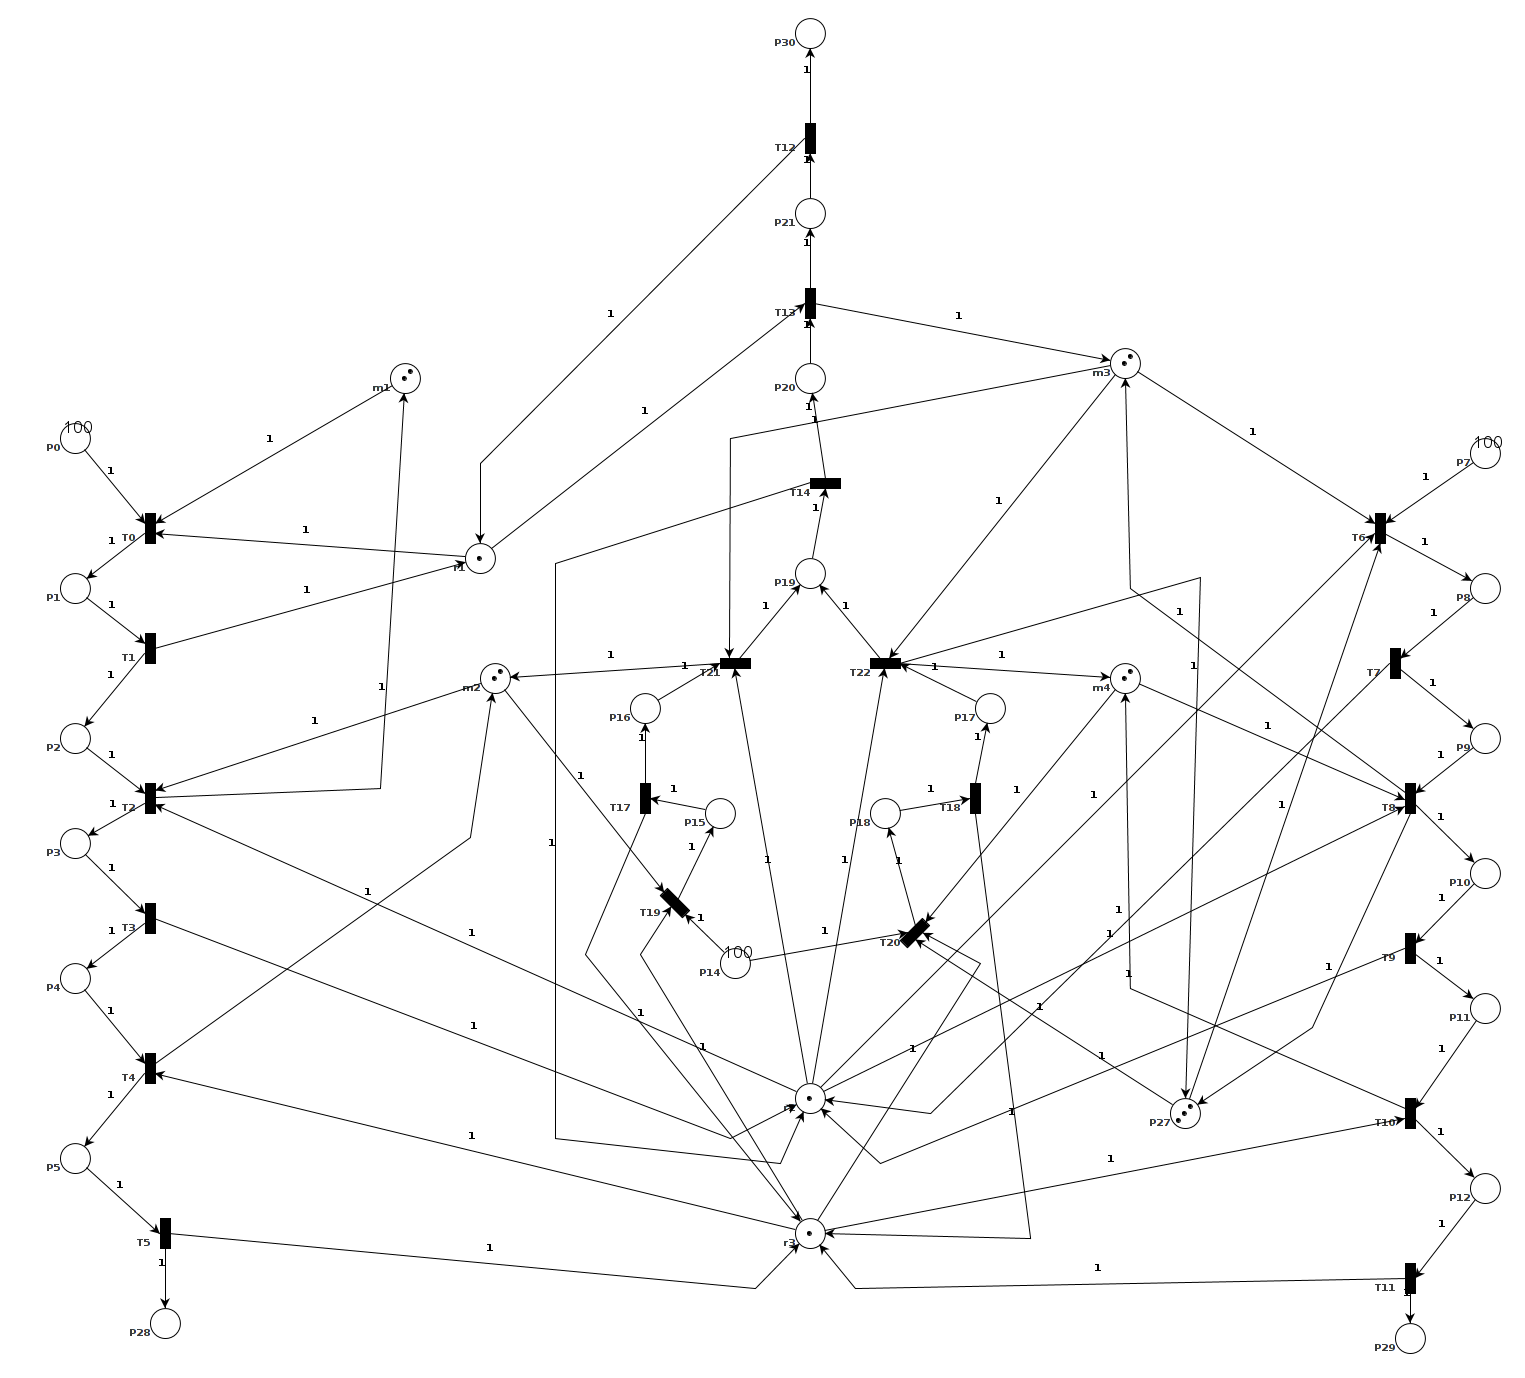
\includegraphics[width=\linewidth]{RedFinal}}
\label{fig:RedFinal}
\end{figure}
%\end{landscape}

\section{Clases}
Con el objetivo de modularizar el código y procurar el encapsulamiento de cada parte, se decidió la implementación de las siguientes clases:
\begin{itemize}
\item Actualizador.java
\item Componente.java
\item FinalConcurrente.java
\item Monitor.java
\item PanelControl.java
\item Proceso.java
\item VentanaPanel.java
\end{itemize}
Se muestra a continuación el diagrama de clases y luego se desarrollará una breve descripción de las clases más importantes y se detallan los métodos más relevantes.
\begin{figure}[H] % Example image
\center{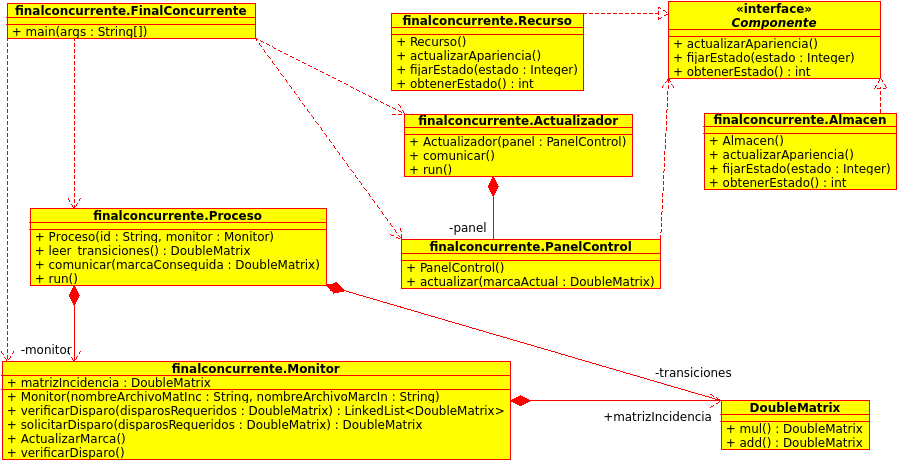
\includegraphics[width=\linewidth]{DiagramaDeClases}}
\label{fig:DiagramaDeClases}
\end{figure}
\subsubsection{Administrador}
Esta clase se encarga de administrar la simulación. Puede ver y modificar absolutamente todos los parámetros de la red Routers, computadoras, conexiones. Tiene la funcionalidad de calcular caminos óptimos con la implementación del algoritmo de Dijkstra para grafos direccionados y que admite ciclos no recurrentes. Adicionalmente es capáz de leer la configuración de la red desde un archivo y dibujar el grafo de la red haciendo uso de la librería graphvz mediante la aplicación dot de los repositorios de ubuntu.
Cabe mensionar que se determinó que todos routers tienen la misma cantidad de maquinas conectadas.
\subsubsection{Arco}
Esta clase representa el arco o la arista de un grafo. Es la entidad que conecta dos nodos o vértices y que se le asigna un peso o distancia.
\subsubsection{Biblioteca\_paquetes}
Esta clase es la estructura de datos que garantiza justicia en el envío de paquetes, esto es, igual atención a las solicitudes de todos los routers y para todas las páginas. En su interiror se implementa una colección de tipo anidada de tres niveles que se usa para organizar los paquetes. Esta colección es del tipo cola y utiliza el campo especial duenio para identificar a qué router y página pertenecen los paquetes encolados.
\subsubsection{Computadora}
Esta clase representa las computadoras o terminales conectadas a los routers en la red a simular. Incluye un puntero al router al que está conectada con el objetivo de solicitarle el envío de una nueva página. Adicionalmente posee una lista de páginas recibidas que podrá ser usada para medir la eficiencia de la red.
\subsubsection{Conexion}
Esta clase representa la vía que comunica dos routers en la red y hace referencia al arco del grafo de la red a simular. Consta de dos nros de ip, el origen y destino así como la especificación del ancho de banda y una cola para emular las limitaciones del canal. 
\subsubsection{Etiqueta}
Esta clase implementa las triplas de tres enteros que utilizará la clase router para determinar hacia dónde debe enviar los paquetes.
\subsubsection{Pagina}
Esta clase representa las páginas que generan las computadoras y que contiene una identificación su tamaño en cantidad de paquetes y las direcciones de origen y de destino en forma de duplas de enteros.
\subsubsection{Paquete}
Esta clase representa las que componen una página y que contiene un número de órden, el tamanio de la página a la que pertenece y las direcciones de origen y de destino en forma de duplas de enteros.
\subsubsection{Router}
Esta clase representa los nodos de la red y opera como enrutador, tiene las funcionalidades de enviar y recibir paquetes así como recibi páginas completas desde las computadoras que están conectadas a este router. La recepción del paquete se realiza mediante la lectura de sus conexiones de recepción y el envío mediante la carga de las conexiones de envío. Cada router tiene una identificación entera, una colección de computadoras, una lista de conexiones de envío y otra de recepción, además cuenta con una tabla de enrutamiento que contiene las etiquetas para cada destino.
%------------------------------------------------

\section{Segunda Fase: Implementación del Algoritmo} % Sub-sub-section
\textit{Algoritmo Implementado: Dijkstra}\\
El algoritmo de Dijkstra resuelve el problema de los caminos más cortos y orígen único en un  grafo dirigido y ponderado $G=(V,E)$ tal que todos los pesos de los arcos son no negativos. Con una buena implementación el timepo de ejecución del algoritmo de Dijkstra es menor al de Bellman-Ford.

\textit{¿Para qué sirve el algoritmo?}\\
La función del algoritmo es calcular los caminos mínimos que hay entre el nodo origen y todos los nodos del grafo.
\textit{¿Cuál es  la lógica del algoritmo?}\\
 El algoritmo parte de un nodo inicial, y se va desplazando a través de  la red, guiándose por los nodos adyacentes al nodo actual. 
Conforme el algoritmo evoluciona se encuentran mejores caminos para determinado nodo destino por lo que se actualiza el resultado. Finalmente el algoritmo termina cuando no quedan nodos sin camino mínimo encontrado.

Dijkstra mantiene un conjunto $S$ de nodos para los que ya se calcularon los caminos mínimos. El algoritmo cíclicamente selecciona un nodo $u \in (V-S)$ cuya distancia es la mínima entre los que quedan sin procesar, agrega el nodo seleccionado $u$ a $S$ y \textsc{ Relaja} todos los vértices adyacentes a $u$.

\begin{leftbar}
\textsc{Dijkstra}(G, nodo\_inicio)\\
1\indent	\textsc{Inicializar}(G)\\
2\indent	$S=\emptyset$\\
3\indent	$Q=G.V$\\
4\indent	\textbf{while} ($Q\neq\emptyset$)\\
5\indent\indent		nodo\_sel=\textsc{Mas Cercano}(Q)\\
6\indent\indent		$S=S\cup nodo\_sel$\\
7\indent\indent		\textbf{for each} $nodo\_i \in G.Adyacentes[nodo\_sel]$\\
8\indent\indent\indent			\textsc{Relajar}(u,v) 
\end{leftbar}

¿Como fue implementada dicha lógica?  Los elementos  que utilizamos son:
\begin{itemize}
\item Conjunto Q: conjunto de nodos no chequeados
\item Conjunto S: conjunto de nodos chequeados
\item Conjunto Adyacentes: conjunto de nodos adyacentes al nodo inicio
\item Vector Predecesores: guarda los valores de los router predecesores a cada router
\item Vector Distancias: almacena las distancias de los caminos mas cortos a cada router
\item Lista de Etiquetas: contiene las etiquetas correspondiente a cada uno de los routers, con los valores en el siguiente formato \\
\verb+{ r_destino, r_siguiente, peso del trayecto }+
\end{itemize}

Primeramente, cargamos en conjunto Q , Adyacentes, las etiquetas, haciendo distinción para la etiqueta del nodo inicio \verb+{ orden_nodo_inicio, 0,0 }+ y las demás \verb+{ orden_nodo_x, -1, INF }+.
Luego recorremos en conjunto Q buscando en las etiquetas de cada uno de los routers, la que contenga el menor trayecto. Con esta condición, seleccionamos el nodo actual o elegido, y lo pasamos al conjunto S.
Luego recorremos los arcos, buscando aquellos que tengan origen en el nodo actual, y que su destino no corresponda a un nodo contenido en S. 
Es entonces, cuando realizamos la comparación de distancias (trayectos almacenados en las etiquetas), con la distancia resultante de la suma de la distancia del trayecto desde el nodo inicio, al nodo actual, las la del trayecto del nodo actual al siguiente para determinar si actualizar o no los valores tanto en el peso de trayectoria, perteneciente a la etiqueta del router siguiente,  como en el Vector Distancias y Predecesores.

Seguidamente, normalizo y actualizo los valores en el Vector Predecesor, con los correspondientes valores de nodos adyacentes al nodo inicio, lo que nos permite posteriormente, armar las tablas para dicho router.
Finalmente, Se actualiza el campo \verb+r_siguiente+ de la etiqueta con el valor correspondiente,  calculado en dicho Vector de Predecesores. Terminando así la ejecución del algoritmo, devolviendo la tabla con los nuevos valores de redireccionamiento.
 
¿Qué diferencia tiene con Floyd-Warshall? Ambos algoritmos tienen la misma finalidad, obtener el calculo del camino mas corto. Pero la diferencia es que Dijkstra calcula los caminos partiendo desde un único nodo base, hasta los demás del grafo, mientras Floyd aplica lo mismo, pero para todos los nodos de la red.
Es decir, si el costo de calculo de Dijkstra es $n \times n$  operaciones, el costo de FFloyd-Warshall será $n \times n \times n$
%------------------------------------------------
\section{Tercera Fase: Pruebas}
Para la validacion del modelo, se realizaron corridas del programa para dos configuraciones con 5,  y 10 routers.
Realizamos capturas de pantallas de (a)Red y (b)Configuración inicial de Arcos para evidenciar la correcta recepción de información a partir del archivo de texto leído.

También capturamos los resultados arrojados por el algoritmo:
(c)en cuanto a distancias $\rightarrow$ (c)Vector Distancia
(d)respecto al router siguiente a direccionar $\rightarrow$ (d)Vector Predecesores
(e)el resultado final para cada router $\rightarrow$ (e)Tablas.

Finalmente, se realiza el seguimiento visual de los paquetes de la página (en amarillo), a lo largo de las conexiones de la red hasta que llega a Destino.

Caso 1: Red de 10 Routers, se realiza el seguimiento de la Pagina 5, de tamaño 5, que se dirige desde el Router 7 al Router 4.

\begin{figure}[H] % Example image
\center{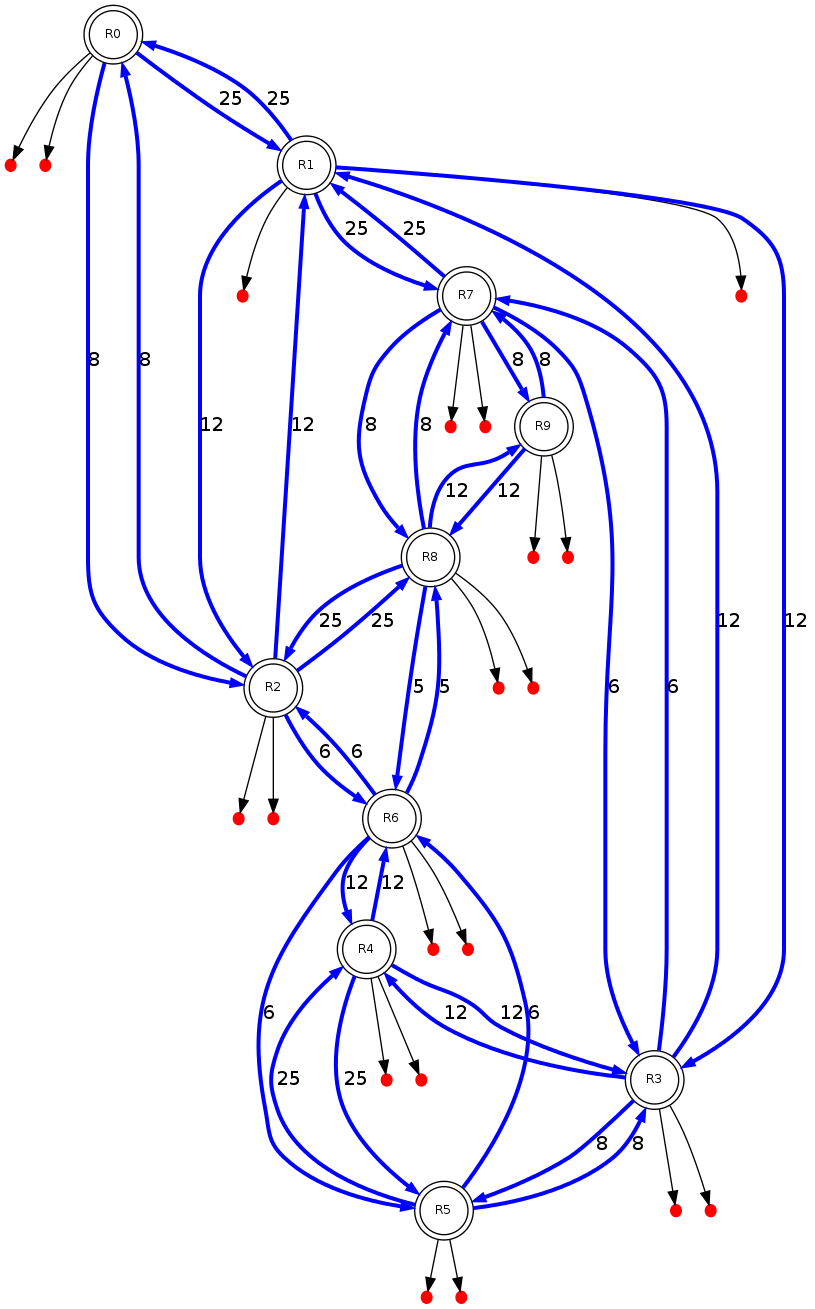
\includegraphics[width=\linewidth]{config_1_A}}
\label{fig:config_1_A}
\end{figure}

\begin{figure}[H] % Example image
\center{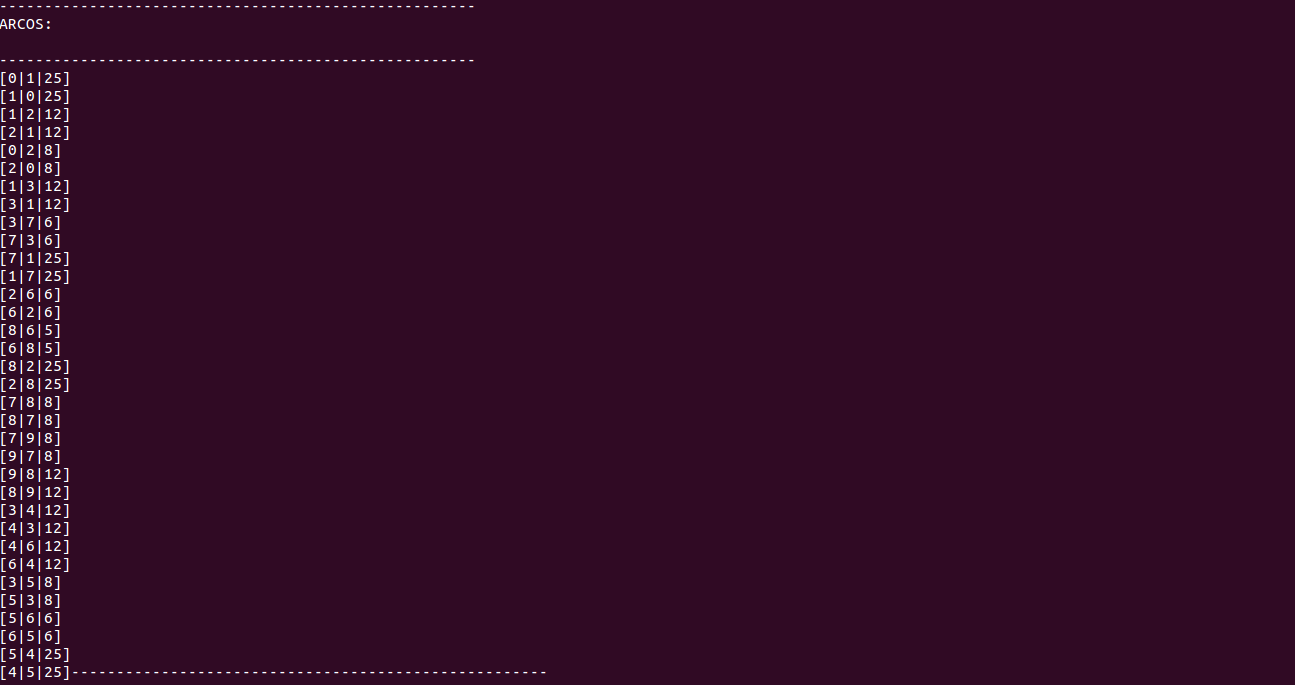
\includegraphics[width=\linewidth]{config_1_B}}
\label{fig:config_1_B}
\end{figure}

La trayectoria del paquete, según dijkstra, será a través de los siguientes routers: 7 $\rightarrow$ 3 $\rightarrow$ 4 con un peso de 18. Lo podemos ver en las tablas calculadas del direccionamiento

\begin{figure}[H] % Example image
\center{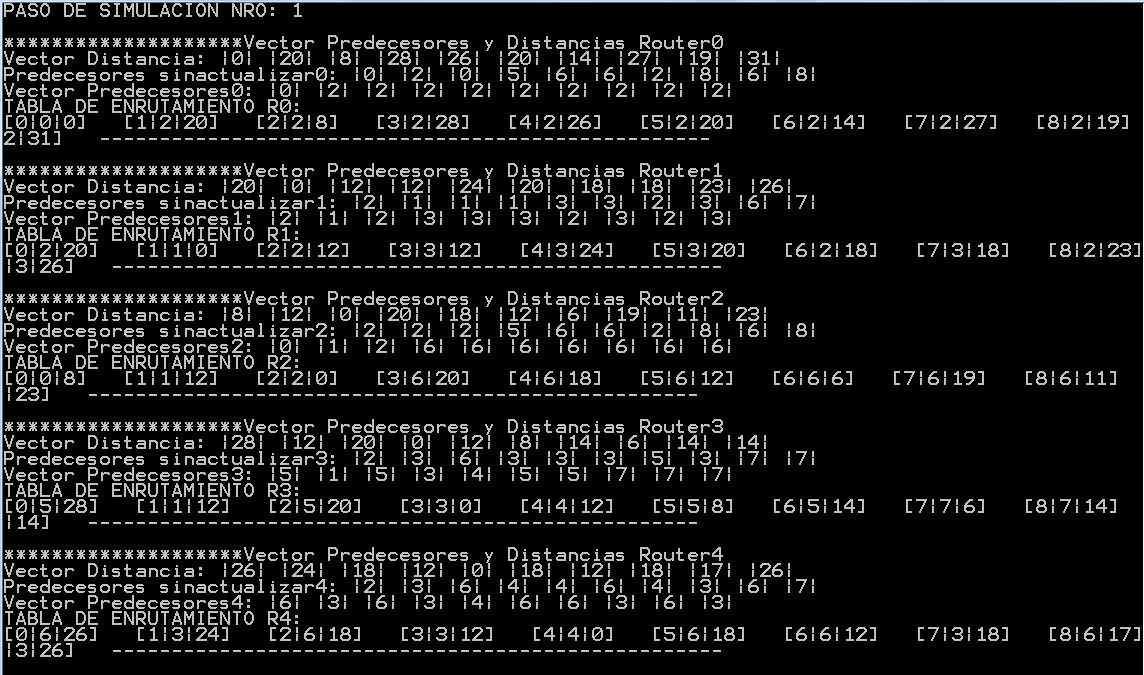
\includegraphics[width=\linewidth]{config1_C_D_y_E}}
\label{fig:config_1_C_D_y_E}
\end{figure}

\begin{figure}[H] % Example image
\center{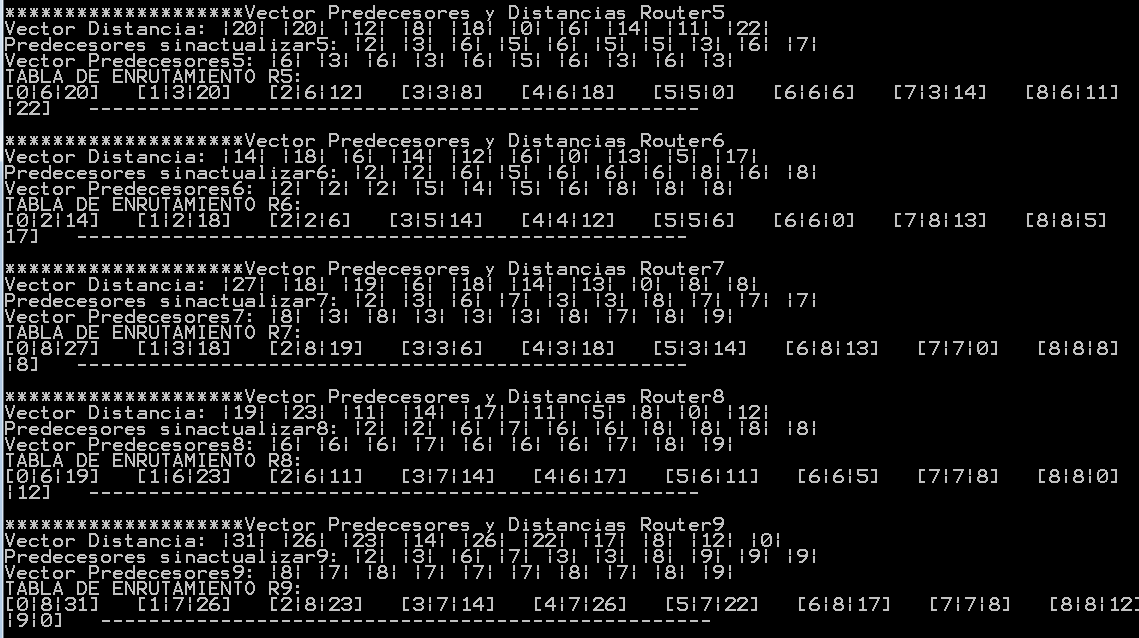
\includegraphics[width=\linewidth]{config1_C_D_y_E_2}}
\label{fig:config_1_C_D_y_E_2}
\end{figure}

Comenzamos el seguimiento de los paquetes de color amarillo.

\begin{figure}[H] % Example image
\center{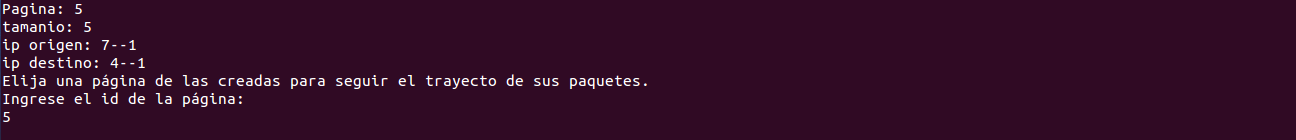
\includegraphics[width=\linewidth]{config_1_run1}}
\label{fig:config_1_run1}
\end{figure}

\begin{figure}[H] % Example image
\center{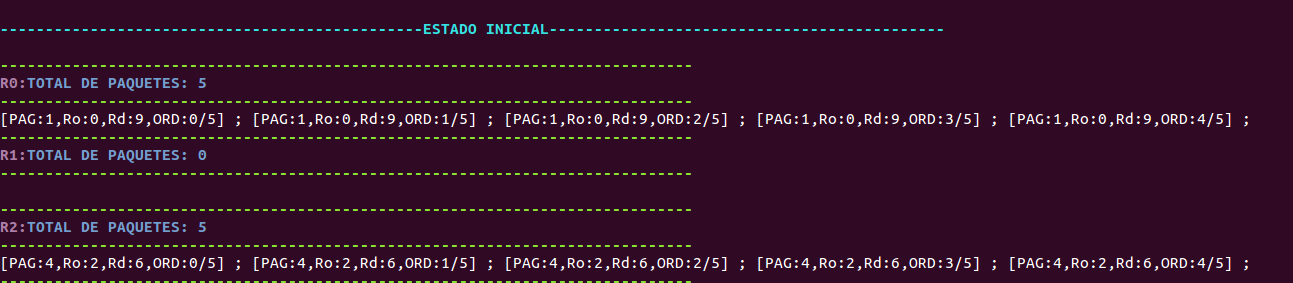
\includegraphics[width=\linewidth]{config_1_run2}}
\label{fig:config_1_run2}
\end{figure}

\begin{figure}[H] % Example image
\center{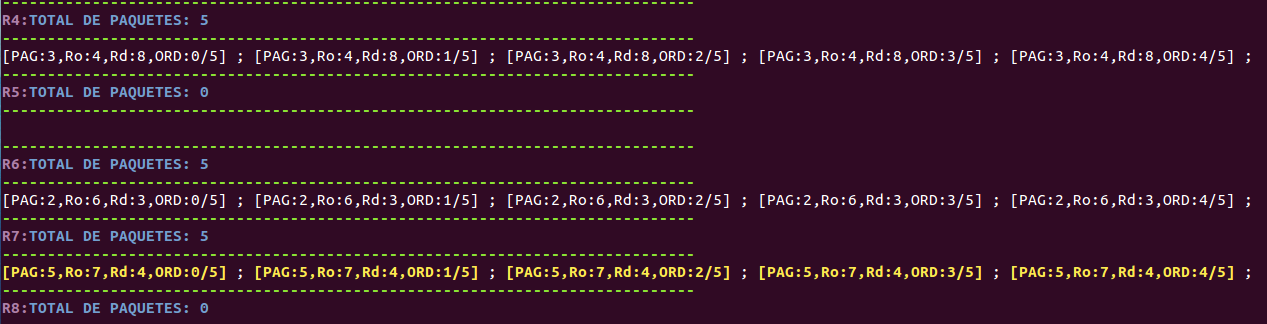
\includegraphics[width=\linewidth]{config_1_run3}}
\label{fig:config_1_run3}
\end{figure}

\begin{figure}[H] % Example image
\center{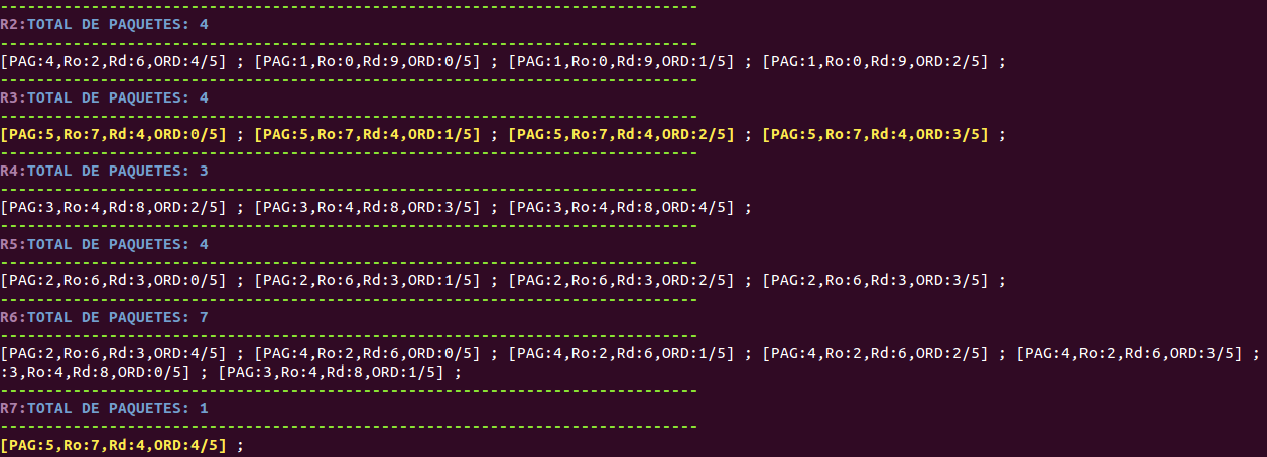
\includegraphics[width=\linewidth]{config_1_run4}}
\label{fig:config_1_run4}
\end{figure}

\begin{figure}[H] % Example image
\center{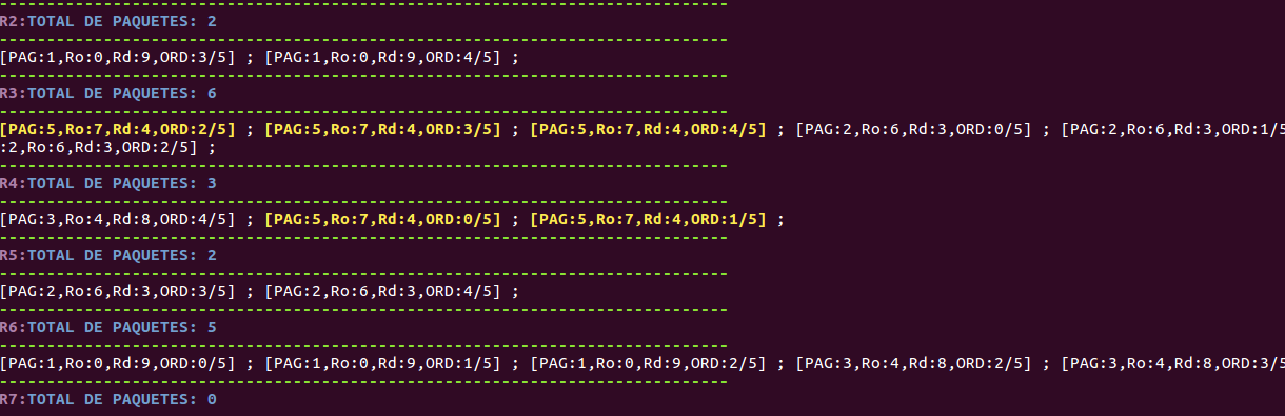
\includegraphics[width=\linewidth]{config_1_run5}}
\label{fig:config_1_run5}
\end{figure}

\begin{figure}[H] % Example image
\center{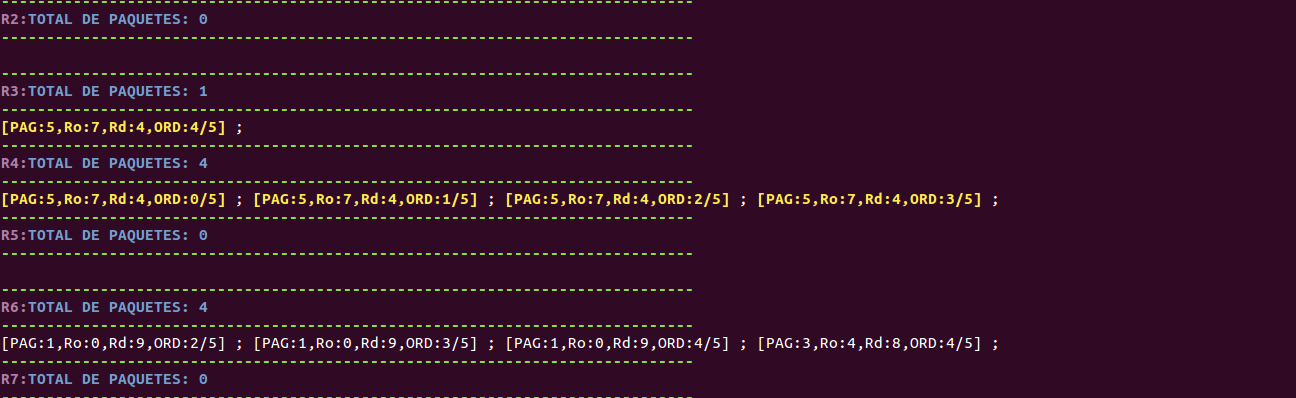
\includegraphics[width=\linewidth]{config_1_run6}}
\label{fig:config_1_run6}
\end{figure}

A consecuencia del ancho de banda de las Conexiones involucradas en la trayectoria y la demanda de paquetes, en 5to pasos de simulación se logra completar la página 5.

\begin{figure}[H] % Example image
\center{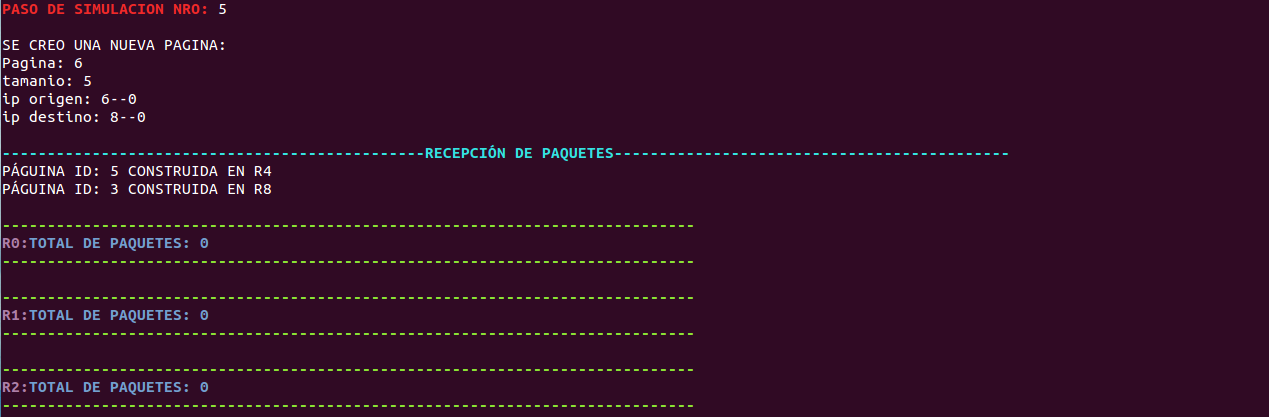
\includegraphics[width=\linewidth]{config_1_run7}}
\label{fig:config_1_run7}
\end{figure}

%----------------------------------------------------------------------------------------
%	CONCLUSION
%----------------------------------------------------------------------------------------

\section{Conclusion} % Major section
Finalizado el desarrollo del trabajo, de la ejecución del algoritmo de dijkstra pudimos apreciar que es una herramienta de gran utilidad y eficiencia.
Aplicamos la propiedad de popularización, junto con un controlador de versiones, la tarea de programación fue más ligera, con el diseño previamente establecido.
Además Pudimos dimensionar la potencialidad de las estructuras utilizadas: Nodo, Lista, Cola, Grafo. Inclusive, fue empleamos la estructura Cola, de manera iterativa, con el fin de conseguir igualdad al momento de selección de paquetes para enviar.
%%\lipsum[12-13]

%----------------------------------------------------------------------------------------
%	BIBLIOGRAPHY
%----------------------------------------------------------------------------------------

\begin{thebibliography}{99} % Bibliography - this is intentionally simple in this template

\bibitem[1]{Figueredo:2009dg}
 \textsc{Cormen, T.~C ; Leiserson, C.E~ ; Rivest, R.L~ } and \textsc{Stein, C~}
\textit{Introduction to Algorithms}, Third Edition
The MIT Press. Cambridge, Massachusetts	London, England, 2009
\newblock {\em Single-Source Shortest Paths}, 24:658--662.

\bibitem[2]{cplusplus.com}
http://www.cplusplus.com/forum/articles/10627/
\textit{Headers and Includes: Why and How} 2009

\bibitem[1]{choorucode.com}
http://choorucode.com/2010/07/22/c-fixing-cyclic-dependencies/
\textit{C++: Fixing Cyclic Dependencies} 2010

\end{thebibliography}

%----------------------------------------------------------------------------------------

\end{document}
